\documentclass{article}
\usepackage{amsmath}
\usepackage{hyperref}
\usepackage{tikz}
\usetikzlibrary{decorations.pathmorphing,patterns}
\usepackage[a4paper]{geometry}
\usepackage{fancyhdr}
\pagestyle{fancy}
\lhead{Der Federoszilator}
\rhead{September 2025}
\begin{document}
 
\section{Federoszilatoren}
\begin{minipage}{\dimexpr\linewidth-4.5cm} 
 Ein \emph{Federoszilator} ist ein Gewicht mit einer Masse $m$, welches über dem Boden durch eine Feder aufgehangen ist. Die gemessene Auslenkung ist dabei die zurückgelegte vertikale Distanz im Vergleich zur Ruheposition. 
 
 Dem \emph{Hookeschen Gesetz} nach ist die rücktreibende Kraft proportional zur Längenänderung, also mit einer Proportionalitätskonstante $D$, der \emph{Federkonstante} oder \emph{Federhärte}
\[
 F = D \cdot \Delta y 
\] 
\end{minipage}
\hfill
\begin{minipage}{4.5cm}
 \center
 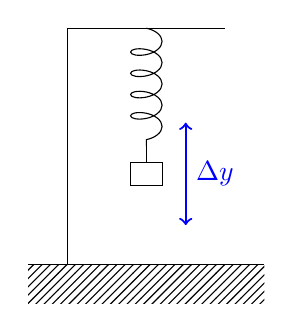
\begin{tikzpicture}
  \fill [pattern = north east lines] (-0.5,-0.5) rectangle (2.5,0);
  \draw (-0.5,0) -- (2.5, 0);
  \draw (0,0) -- (0, 3);
  \draw (0,3) -- (2, 3);  
 
  \draw[decoration={aspect=0.5, segment length=2.7mm, amplitude=2mm,coil},decorate] (1, 3) -- (1, 1.5);
  \draw (1,1.5) -- (1, 1.3); 
  \draw (0.8,1.3) rectangle (1.2, 1);
  
  \draw[<->, blue, thick] (1.5,0.5) -- (1.5, 1.8) node[midway, right] {$\Delta y$}; 
 \end{tikzpicture} 
\end{minipage} 
 
\subsection{Schwingungsdauer} 
Die Schwingungsdauer $T$ eines Federoszilators ist
\[
 T = 2\pi \cdot \sqrt{\frac{m}{D}} 
\]
Dessen Herleitung setzt sich daraus zusammen, dass auf eine $F=D \cdot \Delta y$ eine dem entgegengesetzte Beschleunigung folgt, wobei mit dem Grundgesetz der Mechanik $F=m \cdot a$ gilt. Somit ist
\[
D \cdot y + m \cdot a = 0 
\] 
$a(t)$ folgt daraus, dass die \hyperref[Mechanische Schwingungen]{Schwingungsgleichung} $y(t)$, welche auch eine Strecke $s(t)$ beschreibt, bekannt ist und $s'(t) = v(t)$ und $v'(t) = a(t)$. Somit ist allen \hyperref[Ableitungen]{Ableitungsregeln} nach $y''=a{= -y_{max} \cdot \omega^2 \cdot \sin{(\omega \cdot t)}}$. In die obige Formel eingesetzt und Ausgeklammert folgt
\[ 
 y_{max} \cdot \sin{(\omega \cdot t)} \cdot (D-m \cdot \omega^2) = 0 
\] 
Dem Satz vom Nullprodukt und der offensichtlichen Erkenntnis, dass $y_{max}$ und $\sin{(\ldots)}$ nicht permanent Null sein können, nach folgt dann
\[ 
 D-m \cdot \omega^2 = 0
\]
Wird hier $\omega = \dfrac{2\pi}{T}$ eingesetzt und nach T umgeformt und vereinfacht, folgt
\[
 \boxed{
  T = 2\pi \cdot \sqrt{\frac{m}{D}} 
 } 
\] 
\end{document}